
%% bare_jrnl.tex
%% V1.4b
%% 2015/08/26
%% by Michael Shell
%% see http://www.michaelshell.org/
%% for current contact information.
%%
%% This is a skeleton file demonstrating the use of IEEEtran.cls
%% (requires IEEEtran.cls version 1.8b or later) with an IEEE
%% journal paper.
%%
%% Support sites:
%% http://www.michaelshell.org/tex/ieeetran/
%% http://www.ctan.org/pkg/ieeetran
%% and
%% http://www.ieee.org/

\documentclass[journal]{IEEEtran}

\bibliographystyle{IEEEtran}
\usepackage{lineno,hyperref}
\usepackage{amsmath,graphicx, amssymb,tabularx,booktabs}
\usepackage{subcaption}
\usepackage[font=small,skip=2pt]{caption}
\usepackage{boxedminipage}
%\usepackage{algpseudocode}
%\usepackage{algorithm}
\usepackage{xcolor}
%\usepackage[sort&compress]{natbib}
\usepackage{footnote}
\makesavenoteenv{tabular}



% Example definitions.
% --------------------
\def\x{{\mathbf x}}
\def\L{{\cal L}}


% *** GRAPHICS RELATED PACKAGES ***
%
\ifCLASSINFOpdf
  % \usepackage[pdftex]{graphicx}
  % declare the path(s) where your graphic files are
  % \graphicspath{{../pdf/}{../jpeg/}}
  % and their extensions so you won't have to specify these with
  % every instance of \includegraphics
  % \DeclareGraphicsExtensions{.pdf,.jpeg,.png}
\else
  % or other class option (dvipsone, dvipdf, if not using dvips). graphicx
  % will default to the driver specified in the system graphics.cfg if no
  % driver is specified.
  % \usepackage[dvips]{graphicx}
  % declare the path(s) where your graphic files are
  % \graphicspath{{../eps/}}
  % and their extensions so you won't have to specify these with
  % every instance of \includegraphics
  % \DeclareGraphicsExtensions{.eps}
\fi


% correct bad hyphenation here
%\hyphenation{op-tical net-works semi-conduc-tor}


\begin{document}
%
% paper title
% Titles are generally capitalized except for words such as a, an, and, as,
% at, but, by, for, in, nor, of, on, or, the, to and up, which are usually
% not capitalized unless they are the first or last word of the title.
% Linebreaks \\ can be used within to get better formatting as desired.
% Do not put math or special symbols in the title.
\title{Eliminating object prior-bias from sparse-projection tomographic reconstructions}
%
%
% author names and IEEE memberships
% note positions of commas and nonbreaking spaces ( ~ ) LaTeX will not break
% a structure at a ~ so this keeps an author's name from being broken across
% two lines.
% use \thanks{} to gain access to the first footnote area
% a separate \thanks must be used for each paragraph as LaTeX2e's \thanks
% was not built to handle multiple paragraphs
%

\author{Preeti Gopal,
  Sharat Chandran,
  Imants Svalbe,
        and~Ajit Rajwade
\thanks{Preeti Gopal is with IITB-Monash Research Academy}
\thanks{Sharat Chandran and Ajit Rajwade are with the Department of Computer Science and Engineering, IIT Bombay}
\thanks{Imants Svalbe is with the School of Physics and Astronomy, Monash University}}



% make the title area
\maketitle

% As a general rule, do not put math, special symbols or citations
% in the abstract or keywords.
\begin{abstract}
  Tomographic reconstruction from undersampled measurements is a
  necessity when the measurement process is potentially harmful, needs
  to be rapid, or is resource-expensive. In such cases, information
  from previously existing longitudinal scans of the same object
  (`object-prior') helps in the reconstruction of the current object (`test')  from its
  significantly fewer measurements. A common problem with these techniques is
  the strong influence of object-priors in the reconstruction of new regions in the test.
  In this work, we mitigate this problem by first estimating the location of new regions and
  then imposing object-prior in \textit{only} the other old regions which are similar to the prior.

  Our work is based on longitudinal data acquisition scenarios where
  we wish to study new changes that evolve within an object over time,
  such as in repeated scanning for disease monitoring, or in
  tomography-guided surgical procedures. While this is easily feasible
  when measurements are acquired from a large number of projection
  angles (`views'), it is challenging when the number of views is
  limited (sub-Nyquist). We
  show that in the latter case, a `spatially-varying' technique is
  appropriate in order to prevent the prior from adversely affecting the
  reconstruction of new structures that are absent in any of the
  earlier scans. The reconstruction of new regions is safeguarded from
  the bias of the prior by computing regional weights that moderate
  the local influence of the priors. We are thus able to effectively
  reconstruct both the old and the new structures in the test. We have
  tested the efficacy of our method on synthetic as well as real
  projection data, in both 2D and 3D. Our method
  significantly improves the overall quality of reconstructed data
  while minimizing the number of measurements needed for imaging in
  longitudinal studies.
\end{abstract}

% Note that keywords are not normally used for peerreview papers.
\begin{IEEEkeywords}
Limited-view tomographic reconstruction, regularization priors, object priors, longitudinal studies.
\end{IEEEkeywords}


% For peer review papers, you can put extra information on the cover
% page as needed:
% \ifCLASSOPTIONpeerreview
% \begin{center} \bfseries EDICS Category: 3-BBND \end{center}
% \fi
%
% For peerreview papers, this IEEEtran command inserts a page break and
% creates the second title. It will be ignored for other modes.
\IEEEpeerreviewmaketitle



\section{Introduction}
\label{sec:intro}
Computed Tomography (CT) deals with the recovery of details of an
object's interior
from a limited set of projection data acquired by passing
X-rays at different orientations (`views'). It is preferable to
minimize the radiation exposed in order to prevent any potential
damage to it and in order to reduce the acquisition time. Therefore,
current research seeks to either significantly reduce the radiation
intensity required to reconstruct with adequate
fidelity~\cite{yang2018,Lin2016,Xie2017,gopal2019low} or significantly
reduce the number of measurements required to reconstruct with
adequate fidelity. For the latter case, there are two lines of
pursuit. One is to intelligently choose those sets of projection views
that capture most
information~\cite{King2018,Anthony2018,barkan17,fischer16,andrei14},
and the other, which is the focus of this paper, is to design the
reconstruction algorithm in order to achieve the most accurate
recovery of the underlying slice, given the measurements from any
limited set of views~\cite{yang2018,geyer2015,kilic2011}.

In conventional data acquisition techniques, tomographic
measurements $\boldsymbol{y}$ are acquired by sampling the physical
object $\boldsymbol{x}$ uniformly with a substantial number of views,
ideally above the Nyquist rate. In such a case when there are
sufficient measurements, reconstruction using conventional
filtered backprojection (FBP) suffices, as seen in
Fig.~\ref{fig:story} (first column, 600 views). The figure shows the
ground truth image (260$\times$260) of naturally growing sprouts at the top
left (the details of this dataset is postponed to
Section~\ref{sec:datasets}).

However, reconstruction from reduced views has
been made possible by assuming the data to exhibit certain properties such as
smoothness in image space, sparsity in gradient space~\cite{TV} or sparsity under
certain mathematical transforms~\cite{Donoho,introCS} such as the Discrete Cosine Transform (DCT).  There are multiple such regularization priors and our work aims at significantly improving
the reconstructions obtained from any of these methods. Hence, although our technique is agnostic to the type of regularization prior used, here we have used the total Variation (TV) method as part of our presented solution. If $\boldsymbol{\mathcal{R}}$ represents the acquisition model, then TV-regularized solution is described by one that minimizes a combination of
least squares error and $TV$-norm  of the object $\boldsymbol{x}$. This is described by

 \begin{equation}
   J_{TV}(\boldsymbol{x}) = \lVert\boldsymbol{\mathcal{R}x}- \boldsymbol{y}\rVert_2^2 + \lambda_{TV}TV(\boldsymbol{x})
   \label{Eq:simple_TV}
 \end{equation}

 where the $TV$ norm is given by

  \begin{equation}
   TV(\boldsymbol{x}) = \sum_{i,j}\nabla_{ij}(\boldsymbol{x}).
   \label{Eq:definition_TV}
\end{equation}
 
 Fig.~\ref{fig:story}
 (second column) demonstrates the benefit of using a regularization prior when
 the number of projection views is limited (100 views).
 We solve this cost function using an optimal first-order method for large scale TV regularization
 presented in~\cite{TVReg}  and available in~\cite{TVReg-lib}. 

 %%% Postpone later We observed that there was no significant benefit
 %%% in choosing wavelets over DCT.  }

 \begin{figure}[t]
\centering
	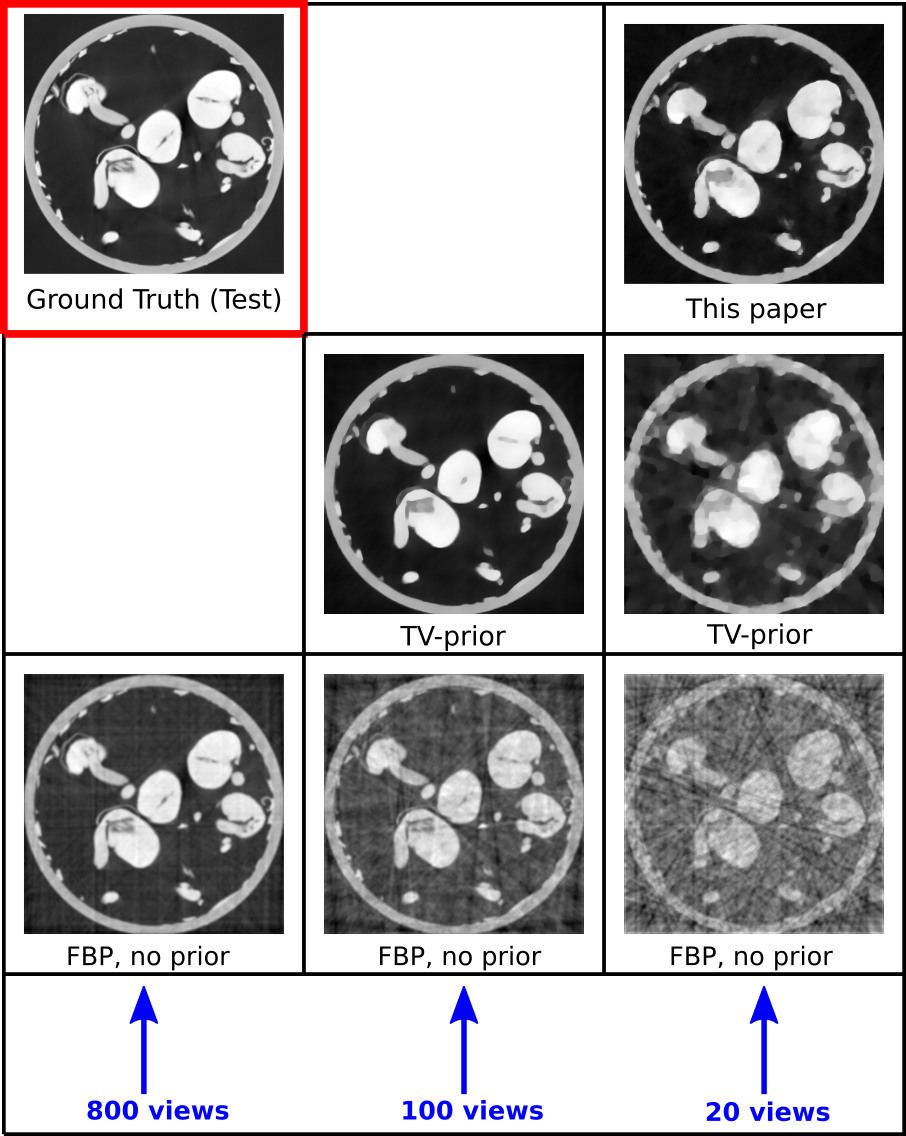
\includegraphics[width=0.45\textwidth]{../images/story/post_TCI/story.png}
        \caption{Illustration of the use of various priors in 
          reconstruction as the number of views reduces. In all cases,
          the ground truth (260$\times$260) appears in the top left.
          For extremely large number of views (800 views), the FBP
          reconstruction (first column) is of very good quality
          (Structural Similarity Index Metric, SSIM=0.92). As the
          number of views become limited (100 views), the
          reconstruction using a general data-independent prior such as Total Variation (TV, middle column) is
          better both visually and quantitatively than FBP (SSIM of
          0.96 vs 0.82). If the number of views is drastically reduced
          (20 views), the presence of both TV prior and object
          prior together improves the reconstruction (SSIM=0.91) when compared
          to presence of only TV prior (SSIM=0.87) or no prior
          (SSIM=0.64).}
 \label{fig:story}
 \end{figure} 

 When the number of views is significantly reduced (this paper), the
 regularization prior alone is not sufficient.  In such cases additional
 information (`object-prior') specific to the current
 object being scanned (called the `test' henceforth) is useful in
 further improving the reconstruction.  While this has been done in
 the context of dynamic CT-scans (discussed more in
 Section~\ref{sec:related}), in this paper we use a set $S$ of
 previous scans of the same object. This is relevant in a longitudinal
 context: the acquisition of sequential CT scans of the same subject
 in order to track time-evolving changes within the subject's
 interior. As seen in Fig.~\ref{fig:story} (last column, 30 views) our
 method uses the set $S$ by creating an
 eigenspace representation (Section~\ref{sec:method_spatially_varying_prior}).

 However, with the use of such an object prior, a new challenge
 emerges. The prior set $S$ may potentially overwhelm the necessary
 details, and when several prior scans are available, finding the
 right prior is an issue. We therefore seek an algorithm that
 estimates the location and magnitude of new changes in the
 (unknown) test. As we show in
 Section~\ref{sec:method_spatially_varying_prior}, this eventually
 prevents the prior from adversely affecting the reconstruction of new
 regions in the test. We refer to this method as a
 \textit{spatially-varying} prior-based reconstruction routine, that
 still uses \textit{all} the previous scans in the set $S$, without
 using the prior scan \textit{as is}, or endeavoring to find the ``right''
 prior.

 This paper is organized as follows. After discussing related work in
 Section~\ref{sec:related}, Section~\ref{sec:contributions} lays down
 the key contributions of this work. Details of the datasets created and
 used for validation
 are described in Section~\ref{sec:datasets}. Section~\ref{sec:tmh}
 demonstrates the utility of our
 method on a longitudinal medical dataset. We now move to the
 details. Section~\ref{sec:method_spatially_varying_prior}
 describes the
 construction of a uniform eigenspace prior and computation of a spatially-varying map in order to preserve new changes in the test. 
 The results of are presented in
 Section~\ref{sec:results_spatially_varying_prior}. Section~\ref{sec:discussion}
 discusses tuning of the hyperparameters involved, and limitations of
 our method. Finally, we conclude with key inferences that can be
 drawn from our work in Section~\ref{sec:conclusions}.
% We present results on real and simulated 3D
%  data for different longitudinal studies.  These are studies wherein
%  sequential CT scans of the same object are acquired to track
%  time-evolving changes within its interior.
 
  %although this optimizer removes most of the artefacts created due to sub-sampling, its reconstruction is blurred when the number of views is very limited, as shown in Fig.~\ref{fig:story2}. 
%(2) there is the key issue of the choice of \textit{a particular} previously scanned object as template among the many previously acquired scans

 \section{Related Work}
 \label{sec:related}
 The idea of using a reduced number of views is most pronounced in
specialized applications. For example, in~\cite{Essam2015},
sparsity-constrained optimization is presented for angiography. Here,
the regions of interest are the vessels alone and they are highlighted
by physically inserting a contrast agent, and therefore there is an
inherent sharper contrast between the vessels and the background.  In
other applications where the spatial-gradient of the underlying volume
is known to be sparse, the `total variation' method, as used
in~\cite{Li2015,Polak2017}, can be applied.  However, as shown earlier
in Fig.~\ref{fig:story}, these regularization priors are not sufficient when very few
views are acquired, thus needing information from stronger priors such as those obtained from previous scans of the same or similar object. 

%  As can be seen
% in the situatiowe will
% later see in Figs.\ref{fig:object-prior_test_okra}
% and~\ref{fig:object-prior_test_sprouts}, the spatial-gradient of many
% datasets is not sparse.

Most object-prior based reconstruction have been in the areas of
dynamic CT and 4D-CT. %In dynamic CT, the object being scanned
%undergoes changes between successive projection views and hence is not
%stationary even within a single complete scan. In contrast, in 4D-CT,
%a set of 3D CT scans are taken over short intervals of time, and the
%object undergoes changes between successive scans.  The reconstruction
%is then performed over the entire set generating several 3D
%volumes.
%In most scenarios, the object-prior
The object-prior usually consists of an object
reconstructed to high quality from a large number of projection
angles. One of the earliest pieces of work in this area is the
well-cited PICCS method~\cite{PICCS} for dynamic CT, which enforces a robust-norm
based similarity between the test and the object prior,
in addition to a sparsity prior on the test. The limitation is the
unchecked over-emphasis of the prior on the reconstruction of the test
at hand. A closely related method called PIRPLE was proposed
in~\cite{pirple}, with additional steps to register the object prior
and the test and a somewhat more flexible combination of data fidelity
terms, sparsity prior and object prior. However, this method too has
similar limitations as PICCS.

In order to prevent the object-prior from overwhelming the
reconstruction of test, a few other approaches have either estimated the
motion between the object-prior and the test or have applied very
specific object-properties for identifying the new changes in the
test.  Examples for the former include~\cite{koen2020}, where the
changes across the successive scan volumes are assumed to be
continuous, thus enabling the use of optical flow to model the motion
between corresponding voxels of different scan volumes. In another
study~\cite{vincent2017}, changes between successive scans were
modelled by affine deformation whose parameters were computed for
motion-correction, which inturn enables acquisition from fewer
views. In~\cite{daniil2015}, all the scan volumes are reconstructed
together using spatio-temporal regularization. Here again, the
inherent assumption is the continuity across volumes in space or
time.

The methods that use object-specific knowledge
are~\cite{Van2015} and~\cite{Marjolein2016}.  In~\cite{Van2015}, the
knowledge of the attenuation coefficient of the fluid is used as a
prior for reconstructing its flow through gravel. However, this relies
on additional expert domain knowledge which may not be available or
which may be infeasible to acquire. Other approaches variously use robust principal components
analysis assuming that the object consists of a large static part
(background) and a sparse moving part (foreground)~\cite{HaoGao},
spline-based models for tracking the regions of change in an SIRT
framework~\cite{Van2014}.

However, all these
techniques~\cite{daniil2015,koen2020,Van2015,HaoGao,Van2014}
essentially reconstruct all the different stages of the object
simultaneously, and use the extra redundancy across time
simultaneously. In the scenario of a longitudinal study (where
projection measurements are acquired at instants that are several
weeks apart) which we consider in this paper, such approaches are not
feasible. A longitudinal study will necessarily require reconstruction
results after acquisition of each set of measurements.

There exists methods for estimating the new changes (in the test)
directly in the projection space. In such techniques which can
be used in longitudinal studies, the object prior
is projected in the same set of views as the current set of test
measurements, and a set of projection differences is computed. These
projection differences are essentially tomographic projections of the
difference between the unknown test and the known object prior. Hence,
a variety of reconstruction algorithms can be used to estimate such a
difference image which can then be added to the object prior to yield
the final estimate of the test. Such methods have been proposed
in~\cite{Pourmorteza2015,Lee2012}. Here the reconstruction of the
difference image will inherently contain sub-sampling artefacts, and
these artefacts will appear in the final reconstruction as there is no
mechanism to mitigate them (unlike the method that we propose). This
can be seen in Sec.~4 of our supplementary material~\cite{supp_paper},
where we have compared our method with~\cite{Lee2012}.

In this paper, we present a technique that makes use of multiple
object priors, corresponding to high quality reconstructions of
similar objects across time, typically in a longitudinal study.
We use these priors to improve the
reconstruction of the test from largely undersampled measurements. In
particular, we define the regions of change between the test and the
eigenspace spanned by the previous high quality object priors in a
purely data driven manner. Additionally, our technique differentiates
between genuine structural changes and ``changes'' that appear due to
undersampling artefacts (as seen in Sec.4 of our supplementary
material~\cite{supp_paper}).  Besides this, since we use a statistical
model with multiple object priors, we avoid the problem of selecting
an appropriate single object prior
unlike~\cite{PICCS,Pourmorteza2015,Lee2012,pirple,Marjolein2016} and
also make use of the additional information available in multiple
priors. Our technique also has the advantage of not requiring any
expert-domain knowledge about the object being scanned.
 
%-------------------------------------------------------------------

\section{Contributions}
\label{sec:contributions}
This paper focusses on few-views reconstruction with an emphasis on
longitudinal studies. In contrast to
the object prior-based studies mentioned above, we
reconstruct the current test object without any assumption of
continuity of changes or some knowledge of the attenuation
coefficients of the structures. We do not make any temporal assumption
in terms of time intervals -- prior scans could be months apart. We
use the current measurements from few-views and previous scans of the
same object. A key idea in our work is the starting point -- the new
test volume is close to the space spanned by the eigenvectors of the
multiple representative previously scanned objects.

% We utilize the uniform global eigenspace prior presented
% in~\cite{my_dicta_paper} which assume 

We also demonstrate how the uniform prior can impose an inflexible
constant weight (and hence an unnecessary bias) when reconstructing
the data. As a solution, we present a method to moderate the control
of the prior by estimating and imposing spatially-varying weights to
the prior in order to reconstruct new structures accurately. This
spatially-varying prior tunes the effect of the templates in different
regions of the reconstruction.

Fig.~\ref{fig:prior_overview} provides an overview.

 %Various forms of object priors have been used for reconstruction from limited views (`few-views'). In ~\cite{Van2014}, the time-varying region within an object is computed by modelling it as a B-spline.
% \cite{PICCS} uses only a single template and enforces a uniform similarity between the current object's reconstruction and the single template. 
%In addition, when some extra information about the object's structure is known~\cite{PICCS,cardiacPICCS,lubner2011,pirple,mota2017},   %The latter limitation was relaxed in~\cite{liu2016,Xu2012} by building dictionary-based priors from multiple previously scanned objects. However, as reported in~\cite{my_dicta_paper}, dictionary priors are not as accurate and fast as global eigenspace priors.

 \begin{figure}[h]
\centering
	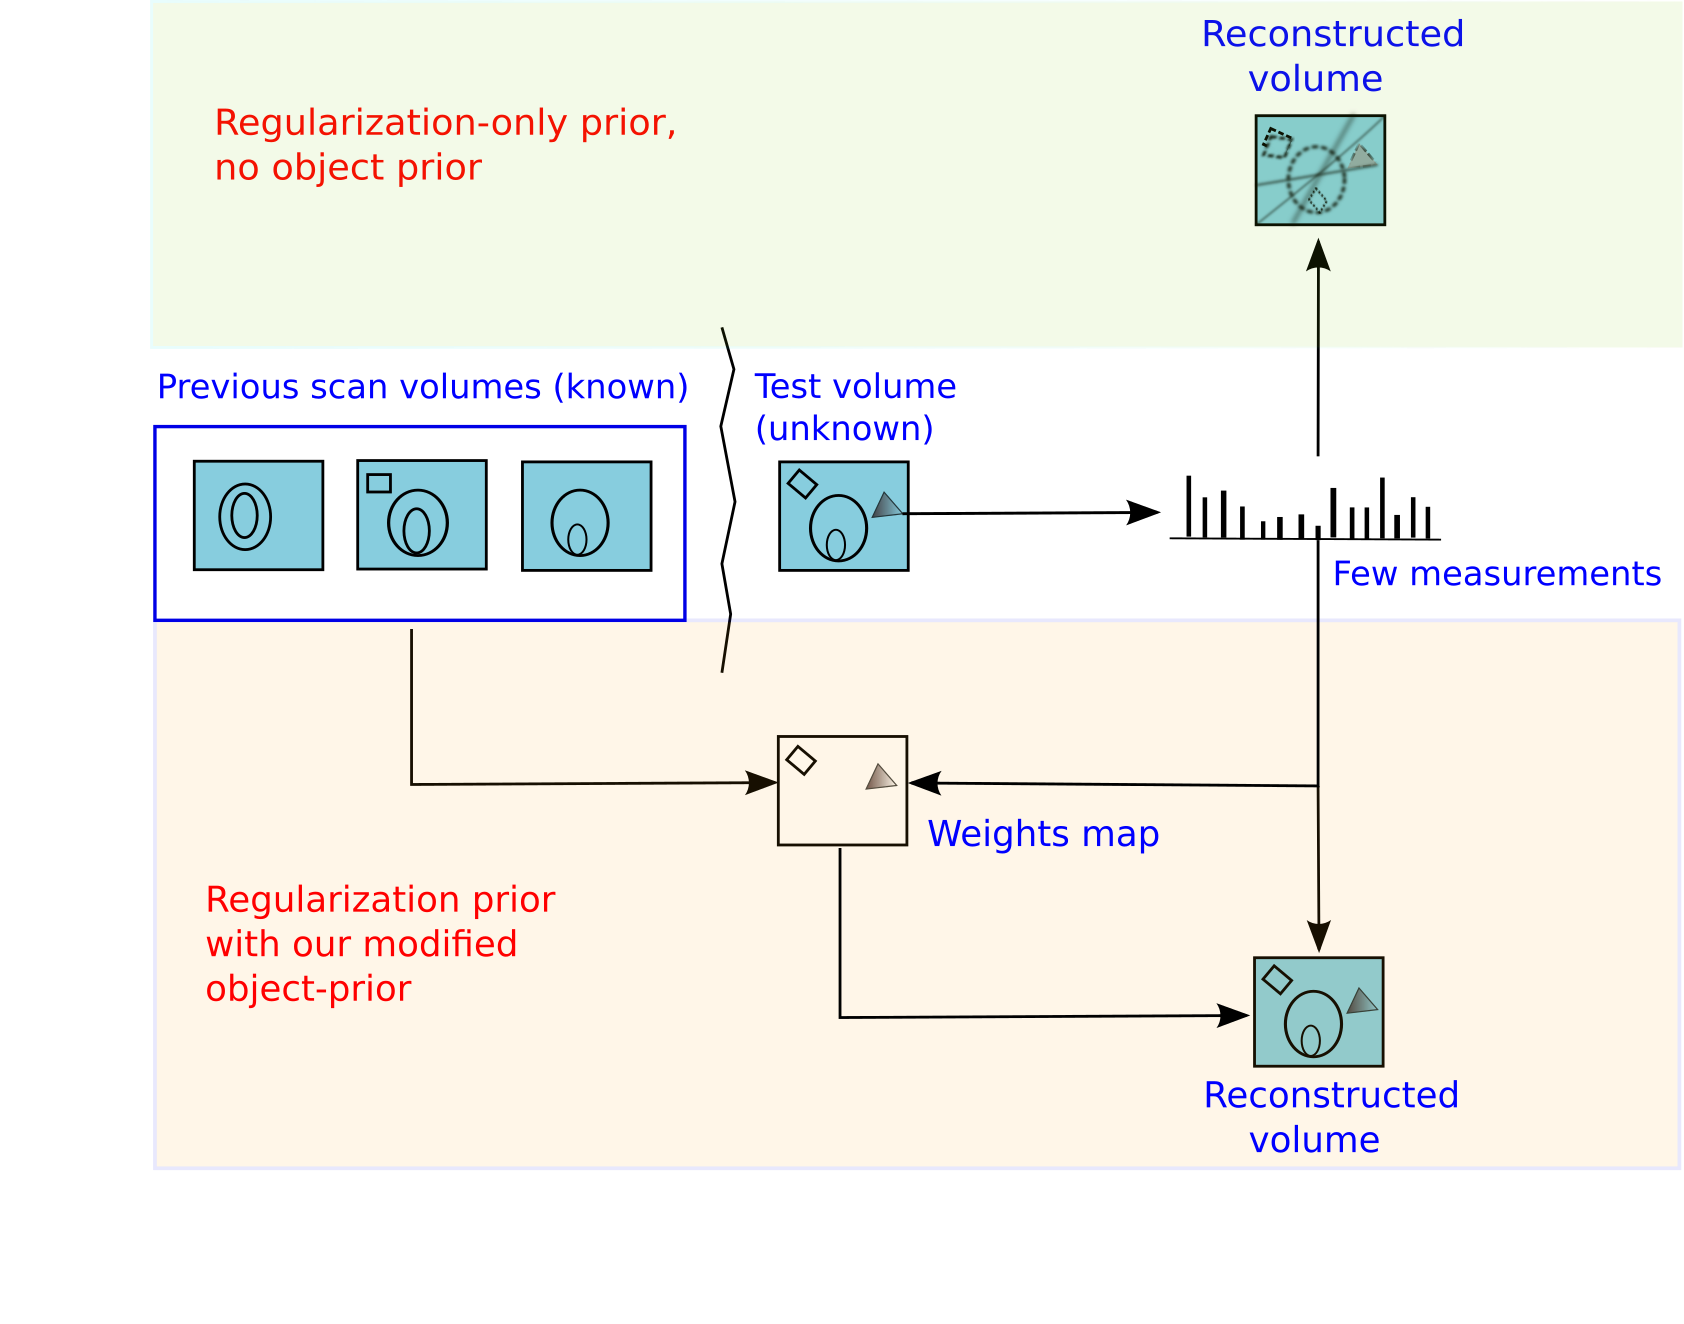
\includegraphics[width=0.5\textwidth]{../images/prior_cmb.png}
        \caption{Overview of our work. When only few measurements are available, the choice of the reconstruction algorithm is driven by availability of object-prior.  (a) In the absence of object-prior, any method that utilizes object-independent prior (such as total variation, sparsity) may be used. (b) In the presence of object-prior, we propose using spatially-varying prior-based reconstruction which utilizes both object-dependent and object-independent priors. In either case, the number of views is lower than what is conventionally used.}
 \label{fig:prior_overview}
\end{figure}

In summary, the key contributions are
\begin{itemize}
\item We create new 3D biological datasets (Section~\ref{sec:datasets}) and
  present results on real cone-beam projections. Our datasets and code
  will be made available to the community.
  \item As seen in Fig.~\ref{fig:story}, we demonstrate the use of
    uniform priors when very few views are used. More results appear
    in Section~\ref{sec:results_uniform_prior} and in the
    supplementary material.
  \item We discuss the scenarios where a uniform object prior is
    sufficient for the application at hand, and the scenarios for
    which it will fail. This leads to the idea of a weights map
    designed to depict the location and strength of new changes at
    every voxel. A novel algorithm is presented to build this map from
    sub-sampled measurements of the test and a set of high quality
    templates. Once the weights map is built, it is used for accurate
    reconstruction of those changes in the test that are absent in all
    of the templates. Results appear in
    Section~\ref{sec:results_spatially_varying_prior}.
  \item We show the efficacy of our results in a real-life medical
    longitudinal studies with data obtained in a clinical setting from
    a live teaching and
    research hospital 
\end{itemize}

%-------------------------------Dataset----------------------------
\section{Datasets}
\label{sec:datasets}
In this section, we lay the details of all the real and simulated
datasets created and used for this work. The first 3 datasets: Okra, Potato and Sprouts were acquired from the Australian National University (ANU). We wish to emphasize that data from commercially
 available CT machines may not be suitable because most CT scanners do
 not reveal the raw measurements, and instead output only the full
 reconstructed volumes. Moreover, the process of conversion from the
 projections to the full volumes is proprietary. Departing from this, we
 demonstrate reconstruction results (in Sections~\ref{sec:results_uniform_prior} and~\ref{sec:results_spatially_varying_prior} from the following datasets.\\

 \textbf{Okra:} This dataset is that of an Okra specimen consisting of its five
scans (Fig.~\ref{fig:object-prior_test_okra}). Prior to the first scan, two cuts were
drilled on the surface of the specimen. This was followed by four
scans, each after introducing one new cut. The specimen was kept in
the same position throughout the acquisitions. The measurements
consisted of real circular cone-beam projections from 450 views, each of size
336$\times$156. 
%In cases where such an
%alignment is not present, all the template volumes must be pre-aligned
%before computing the eigenspace. The test must be registered to the
%object-prior after its preliminary pilot reconstruction.
In our experiments, the first 4 volumes shown in Fig.~\ref{fig:object-prior_test_okra} were used to build the object-prior and the
last volume was used as the test. The ground truth
consists of volumes of size 338$\times$338$\times$123 reconstructed
using the Feldkamp-Davis-Kress (FDK) algorithm~\cite{FDK} from the
full set of 450 view projections.
\\
 %--------------------------------okra data-------------------------------
\begin{figure}[!h]
  \begin{subfigure}[b]{0.18\linewidth}
        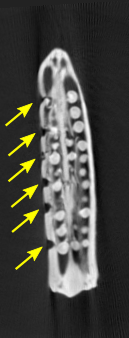
\includegraphics[width=\textwidth]{../images/okra/template4_marked.png}
\captionsetup{labelformat=empty}
        \caption{}
  \end{subfigure}
  \begin{subfigure}[b]{0.18\linewidth}
        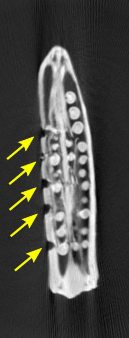
\includegraphics[width=\textwidth]{../images/okra/template3_marked.png}
\captionsetup{labelformat=empty}
        \caption{}
     \end{subfigure}
    \begin{subfigure}[b]{0.18\linewidth}
        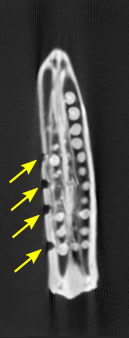
\includegraphics[width=\textwidth]{../images/okra/template2_marked.png}
\captionsetup{labelformat=empty}
        \caption{}
    \end{subfigure}
     \begin{subfigure}[b]{0.18\linewidth}
        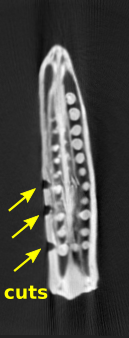
\includegraphics[width=\textwidth]{../images/okra/template1_marked.png}
\captionsetup{labelformat=empty}       
 \caption{}
    \end{subfigure}
     \begin{subfigure}[b]{0.176\linewidth}
        \fcolorbox{white}{blue}{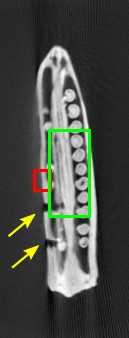
\includegraphics[width=\textwidth]{../images/okra/test_marked.png}}
\captionsetup{labelformat=empty}
        \caption{}
    \end{subfigure}
     \caption{Okra 3D dataset: One slice each from the scanned objects that are used as object-prior (the first four from left) and a slice from the test 
        volume (extreme right). Notice the regions marked in red and green boxes; while all slices have deformities, the test has none.}
\label{fig:object-prior_test_okra}
\end{figure}
%----------------------------------------------------

\textbf{Potato:} This dataset consisted of four scans of the humble potato (Fig.~\ref{fig:object-prior_test_potato_A}). While the first scan was taken of the undistorted potato, subsequent scans were taken of the same specimen, each time after drilling a new hole halfway into the potato. Measurements from each scan consisted of real circular cone-beam projections from 900 views, each of size 150$\times$150. %Further, this alignment can be refined following every update of the reconstructed test volume.
In our experiments, the first 3 volumes were used to build the object-prior and the
last volume was used as the test. The ground truth consists of volumes of size 150$\times$150$\times$100 reconstructed using FDK from the full set of 900 projection views. 
%---------------------------------------
\begin{figure}[!h]
    \begin{subfigure}[b]{0.24\linewidth}
        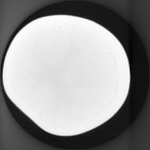
\includegraphics[width=\textwidth]{../images/potato/template_1.png}
\captionsetup{labelformat=empty}       
 \caption{}
    \end{subfigure}
    \begin{subfigure}[b]{0.24\linewidth}
        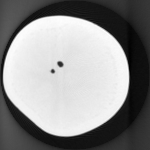
\includegraphics[width=\textwidth]{../images/potato/template_2.png}
\captionsetup{labelformat=empty}
        \caption{}
     \end{subfigure}
    \begin{subfigure}[b]{0.24\linewidth}
        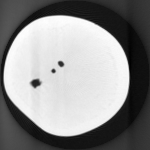
\includegraphics[width=\textwidth]{../images/potato/template_3.png}
\captionsetup{labelformat=empty}
        \caption{}
     \end{subfigure}
    \begin{subfigure}[b]{0.235\linewidth}
        \fcolorbox{blue}{blue}{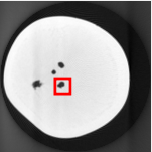
\includegraphics[width=\textwidth]{../images/potato/testIm_color.png}}
\captionsetup{labelformat=empty}
\caption{}
\label{fig:potato3D_test}
     \end{subfigure}
      \caption{Potato 3D dataset: One slice each from the previously scanned objects (the first three from left) and a slice from the test 
        volume (extreme right). Notice the appearance of the fourth
        hole in the test slice. }
\label{fig:object-prior_test_potato_A}
\end{figure}

%\subsection{Simulated measurements from real-life reconstructed volumes}
\textbf{Sprouts:} This 3D dataset, which was also obtained at ANU,
consists of six reconstructed volumes corresponding to six scans of an
in-vivo sprout specimen imaged at its various stages of growth
(Fig.~\ref{fig:object-prior_test_sprouts}).  \textit{In contrast to the
scientific experiment performed for the case of the okra and potato
where we introduced man-made defects, the changes here are purely the
work of nature.} In our experiments, the first 5 volumes were used to build the object-prior and the last volume was used as the test. The ground truth consists of FDK reconstructed
volumes of size 130$\times$130$\times$130 from a set of 1800 view
projections. For the test, cone-beam projections were generated from
the test volume. \\
%-------------------------sprouts data

\begin{figure}[!h]
    \begin{subfigure}[b]{0.3\linewidth}
        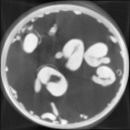
\includegraphics[width=\textwidth]{../images/sprouts/template_1.png}
\captionsetup{labelformat=empty}
        \caption{}
    \end{subfigure}
\quad
    \begin{subfigure}[b]{0.3\linewidth}
        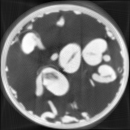
\includegraphics[width=\textwidth]{../images/sprouts/template_2.png}
\captionsetup{labelformat=empty}
        \caption{}
     \end{subfigure}
\quad
    \begin{subfigure}[b]{0.3\linewidth}
        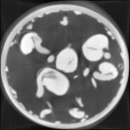
\includegraphics[width=\textwidth]{../images/sprouts/template_3.png}
\captionsetup{labelformat=empty}
        \caption{}
     \end{subfigure}\\
    \begin{subfigure}[b]{0.3\linewidth}
        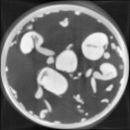
\includegraphics[width=\textwidth]{../images/sprouts/template_4.png}
\captionsetup{labelformat=empty}
        \caption{}
     \end{subfigure}
\quad
    \begin{subfigure}[b]{0.3\linewidth}
        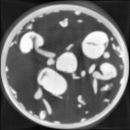
\includegraphics[width=\textwidth]{../images/sprouts/template_5.png}
\captionsetup{labelformat=empty}
        \caption{}
     \end{subfigure}
\quad
    \begin{subfigure}[b]{0.29\linewidth}
        \fcolorbox{blue}{blue}{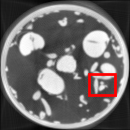
\includegraphics[width=\textwidth]{../images/sprouts/testIm_red.png}}
\captionsetup{labelformat=empty}
        \caption{}
     \end{subfigure}
      \caption{Sprouts 3D dataset: One slice each from the previously scanned objects (the first five from left) and a slice from the test (extreme
        right). Notice the structure within the red box in the test that is different from all of the other images.}
\label{fig:object-prior_test_sprouts}
\addtolength{\textfloatsep}{-0.8cm}
\end{figure}

\textbf{Liver:} %We have used this dataset
 %to illustrate an application
%where \textit{both} uniform and spatially-varying priors are
%useful.
This data was sourced from Tata Memorial Centre~\cite{tmh} in Parel,
Mumbai.  This is the national comprehensive centre for the prevention,
treatment, education and research in cancer, and is recognized as one
of the leading cancer centres in India. The dataset
(Fig.~\ref{fig:RFA2_test_object-prior}) from this longitudinal medical
study consists of 8 scans taken at different stages of radio-frequency
ablation study of a liver. In such a procedure~\cite{Dong2015}, the
physician inserts a thin needle-like probe into the organ. Repeated CT
scans of the patient are acquired in order to track the movement of
the needle and to ensure that it is reaching the appropriate target
tumor. Once the needle hits the tumor, a high-frequency electric
current is passed through the tip of the probe and this burns the
malignant tumor (ablation). The aim of the scan at this ablation stage
is to reveal accurate details of the changes within.

In our experiments, we generate parallel beam measurements from 2D
slices from each of the 8 volumes. Note that all these 8 slices are
located at the \emph{same} index (slice number corresponding to the
same depth) within each of the respective volumes.  Observe (in
Fig.~\ref{fig:RFA2_test_object-prior}) that the needle is seen in all
of the first 7 slices and the effect of ablation is seen in the 8th
slice.
%In our experiments using this dataset, we demonstrate the usefulness of \textit{both} uniform prior and spatially varying prior. For the first case, we choose the first 6 slices to build the object prior and use slice 7 as the test. For the latter case, we choose the first 7 slices to build the object prior and use slice 8 as the test.
%--------------------------Results on TMH data--------------------------
%------------------RFA 2 data
\begin{figure}[h!]
    \begin{subfigure}[b]{0.24\linewidth}
        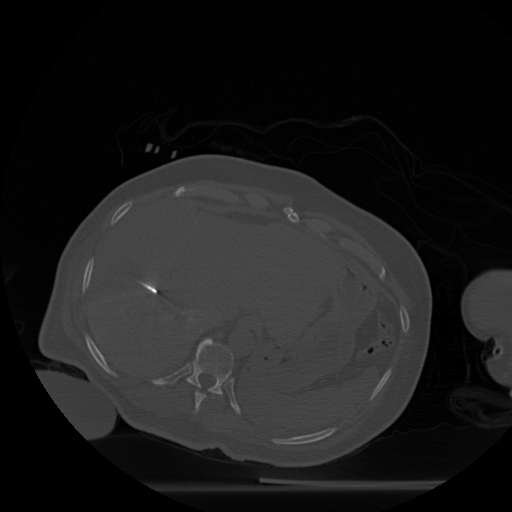
\includegraphics[width=\textwidth]{../images/tmh/RFA2/template1.png}
%\captionsetup{labelformat=empty}       
 \caption{slice 1}
    \end{subfigure}
    \begin{subfigure}[b]{0.24\linewidth}
        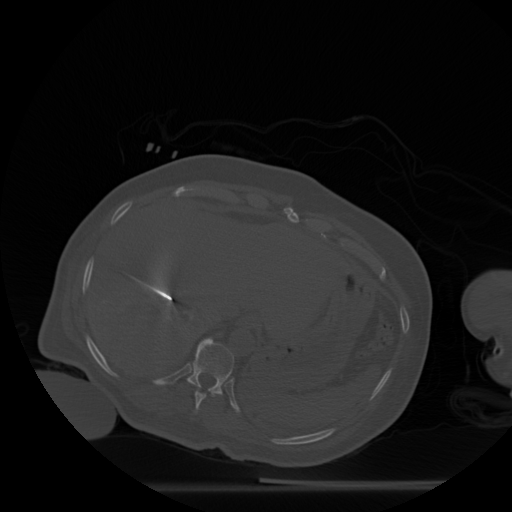
\includegraphics[width=\textwidth]{../images/tmh/RFA2/template2.png}
%\captionsetup{labelformat=empty}       
 \caption{slice 2}
    \end{subfigure}
     \begin{subfigure}[b]{0.24\linewidth}
        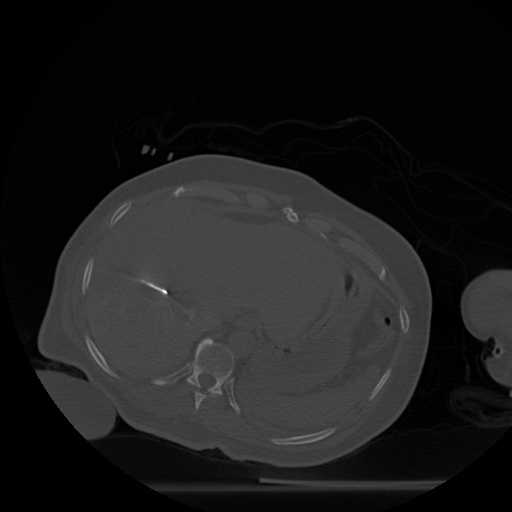
\includegraphics[width=\textwidth]{../images/tmh/RFA2/template3.png}
%\captionsetup{labelformat=empty}       
 \caption{slice 3}
    \end{subfigure}
       \begin{subfigure}[b]{0.24\linewidth}
        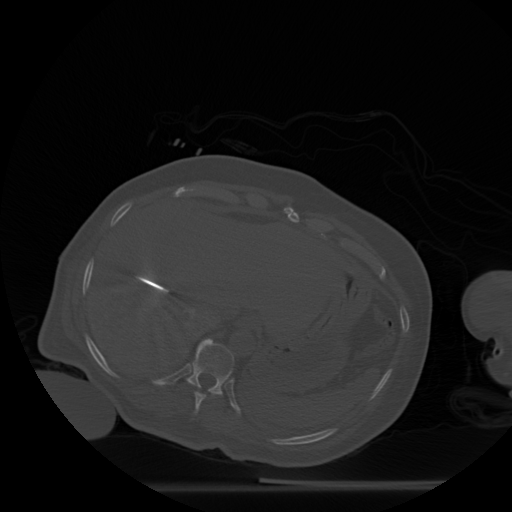
\includegraphics[width=\textwidth]{../images/tmh/RFA2/template4.png}
%\captionsetup{labelformat=empty}       
 \caption{slice 4}
    \end{subfigure}
       \begin{subfigure}[b]{0.24\linewidth}
        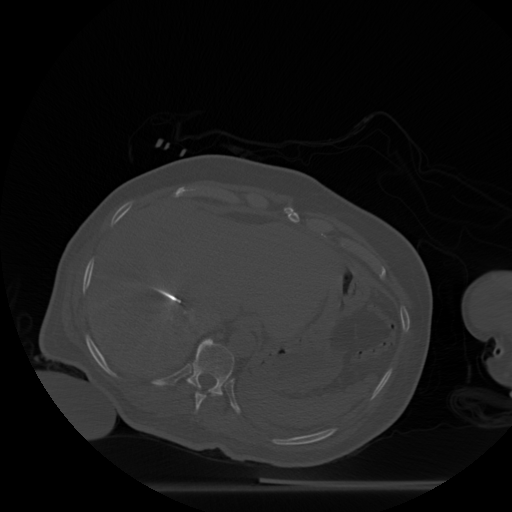
\includegraphics[width=\textwidth]{../images/tmh/RFA2/template5.png}
%\captionsetup{labelformat=empty}       
 \caption{slice 5}
    \end{subfigure}
              \begin{subfigure}[b]{0.24\linewidth}
        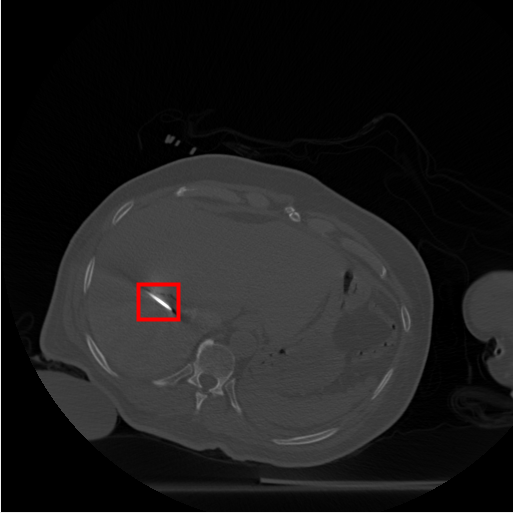
\includegraphics[width=\textwidth]{../images/tmh/RFA2/template6_color.png}
%\captionsetup{labelformat=empty}       
 \caption{slice 6}
    \end{subfigure}
       \begin{subfigure}[b]{0.23\linewidth}
        \fcolorbox{white}{blue}{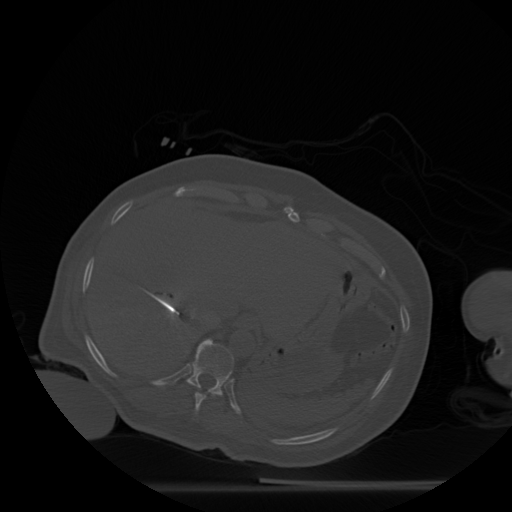
\includegraphics[width=\textwidth]{../images/tmh/RFA2/template7.png}}
%\captionsetup{labelformat=empty}       
 \caption{slice 7}
    \end{subfigure}     
     \caption{Radio-frequency ablation dataset: One of the slices (512$\times$512) from each of the 7 scan volumes of a longitudinal study dataset of the liver. Note that in volumes (a) through (g), the needle (shown in red in (f)) approaches the target tumor.} 
\label{fig:RFA2_test_object-prior}
\end{figure}

%--------------------------------THM section-------------------------
\section{Application: Reconstruction for CT-guided radio-ablation study}
\label{sec:tmh}
Before diving into the details of the uniform and the
spatially-varying prior methods, we first show how \textit{both} the
techniques can be applied to our advantage in a real-life medical
longitudinal study. Here, our data consists of successive scans of the liver taken
during a radio-frequency ablation procedure as described in Sec.~\ref{sec:datasets}. In this context, we classify the goal of any of our
reconstruction techniques into two categories: 
\begin{enumerate}
\item to track the position of the needle, and% in a relatively well-reconstructed background.%Initially, when our goal is to only track the location of the probe while simultaneously reducing sub-sampling artefacts, we advocate capturing measurements from a small number of views (`few-view' imaging) and using uniform prior based reconstruction.
\item to accurately observe the new changes when the needle touches the tumor,%Later, when the probe is proximal to or touches the tumor, our goal is to observe details of tumor ablation while simultaneously reducing sub-sampling artefacts. In this case, we propose to capture measurements from a slightly higher number of views (`moderate-view' imaging) to acquire more information, and use a spatially-varying prior-based reconstruction. The spatially-varying technique moderates the effect of the prior in the reconstruction of new changes in the object being scanned.
\end{enumerate}
while simultaneously reducing the sub-sampling artefacts.
%Here, we demonstrate the combined use of l1-ls (CS) with the object
%prior, in two flavors: the vanilla (uniform) and spatially-varying
%prior-based reconstruction.
The choice of the number of
measurement views and the type of reconstruction -- uniform or
spatially-varying, is driven by the goal of the procedure. First, in
order to track the needle, a very small number of views is sufficient
because the needle has a very high attenuation coefficient when
compared to that of the organs. We use the uniform prior
reconstruction here to reduce the artefacts due to sub-sampling. The
uniform method is fast and sufficient to track the position of the
needle.  Once the needle reaches the site of the tumor, we propose
changing the imaging protocol to acquire measurements from a moderate
number of views. This will enable us to get more information about the
new changes. In addition, we then deploy the spatially-varying prior
method in order to locate the regions of new changes and penalize any
dominance of the prior in these regions.  Regardless of the imaging
protocol we use (`few' or `moderate'), the number of views is smaller
(atleast one-fifth) than the conventional number of views used in a
standard hospital setting. To summarize, when our aim is\\
\begin{itemize}
\item \textbf{Tracking the needle},  we first choose slices 1-6 as our
object-prior, and reconstruct slice 7 with the specific goal of
tracking the needle and simultaneously reduce
artefacts. Fig.~\ref{fig:RFA2_very_few_views} shows the reconstruction
of slice 7 from its measurements from only 90 views. The
reconstructions are quantitatively compared using SSIM.
\end{itemize}
%--------------------RFA 2 few views
\begin{figure}[!h]
\centering
\subcaptionbox{Test}{\fcolorbox{white}{green}{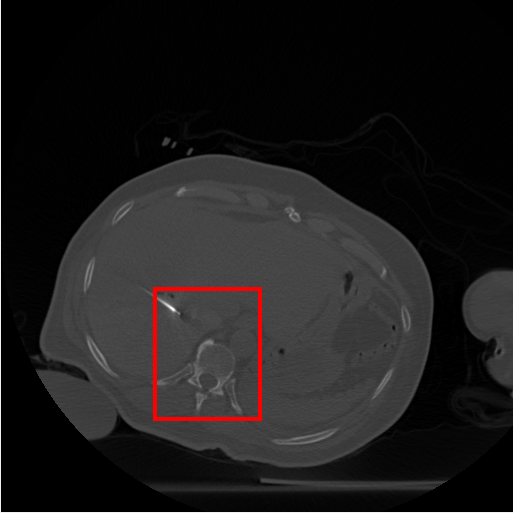
\includegraphics[width=0.23\columnwidth]{../images/tmh/RFA2/post_TCI/very_few_views/colorTestIm.png}}}\hfill
\subcaptionbox{FBP}{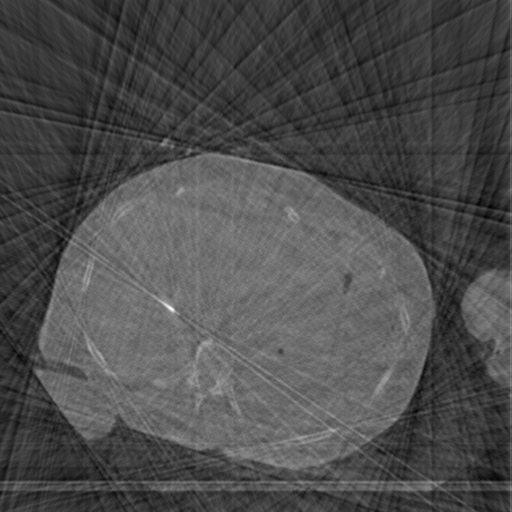
\includegraphics[width=0.24\columnwidth]{../images/tmh/RFA2/post_TCI/very_few_views/fbp.png}}\hfill
\subcaptionbox{TV}{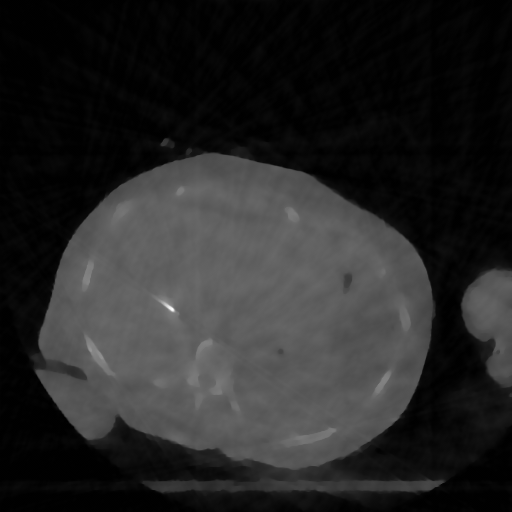
\includegraphics[width=0.24\columnwidth]{../images/tmh/RFA2/post_TCI/very_few_views/tv_lambdaTV_0.036.png}}\hfill
\subcaptionbox{Spatially\\varying prior}{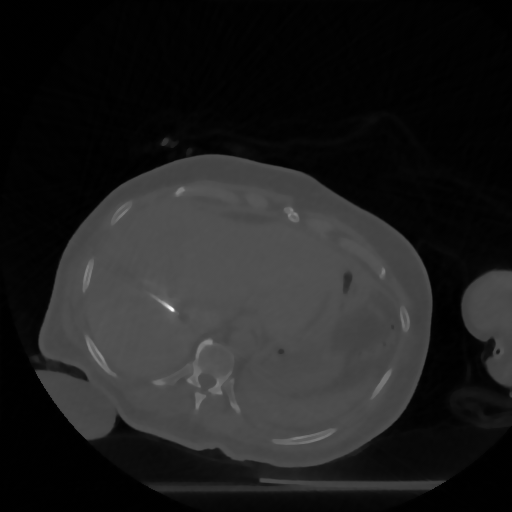
\includegraphics[width=0.24\columnwidth]{../images/tmh/RFA2/post_TCI/very_few_views/weighted_prior_kk_30_lambda_prior_1.100000.png}}
\subcaptionbox{Weights map}{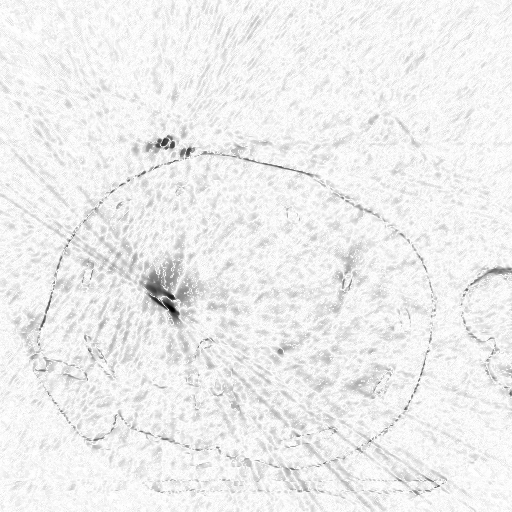
\includegraphics[width=0.24\columnwidth]{../images/tmh/RFA2/post_TCI/very_few_views/weightsIm_kk_30_lambda_prior_1.100000.png}}
\caption{\small{ Reconstruction of `test' (slice 7) from Fig.~\ref{fig:RFA2_test_object-prior} from only 30 views, using (b) FBP and no prior resulting in streaks, SSIM=0.73 (c) TV resulting in blurred bone structures, SSIM=0.91 and (d) spatially varying object-prior (slices 1-6 of Fig.~\ref{fig:RFA2_test_object-prior} are used as object-prior) resulting in clear bone structures with less streaks, SSIM=0.95. The region enclosed in red rectangle is our Region of Interest (RoI) as it contains both the new position of the needle and some background. All SSIM values are computed for this RoI. (e) shows the computed weights map (defined later in the paper) used for reconstruction. Darker intensities indicate lower weights to prior as these are the regions of new changes.}}
\label{fig:RFA2_very_few_views}
\end{figure}


%---------------------------------Uniform section---------------------
\section{Spatially-Varying prior-based reconstruction}
\label{sec:method_spatially_varying_prior}
Having presented the application, we first review the algorithm~\cite{my_dicta_paper} for a uniform  prior-based reconstruction since we are extending this algorithm to 3D reconstructions as part of this work.
%Principal Component Analysis (PCA) has been traditionally used to find the significant modes of (Gaussian corrupted) data. In this regard, it has been widely applied in the context of data compression. However, PCA can also be seen as a tool to provide an orthogonal basis to represent the space in which most of the test data could lie (except the new changes). This space is constructed from the available set of previously scanned objects which must cover a realistically representative range of structures. %, which was shown~\cite{my_dicta_paper} to be better when compared to dictionary-based priors. %A preliminary version of this particular method was earlier presented in \cite{my_dicta_paper}. 
We first present the eigenspace-cum-CS prior-based reconstruction. To begin with, when an object is scanned multiple times, a set of high quality reconstructions (i.e., reconstructions from a dense set of projection views) may be chosen as object-prior for the reconstruction of future scan volumes, which in turn, may be scanned using far fewer measurements. The eigenspace $E_{\text{high}}$ of the $L$ previously scanned objects $Q_1,Q_2,...,Q_L$ is pre-computed. Here, it is assumed that most of the test volume, barring the new changes, can be expressed as a sparse linear combination of the principal components (eigenvectors of the covariance matrix) obtained from a group of structurally similar volumes. Hence, the object-prior is represented by means of PCA. For the eigenspace to encompass a range of possible structures in the test slice, the object-prior must represent a wide structural range. Moreover, if these volumes are not aligned, then they must be first registered before computing the prior. The prior is built by computing the covariance matrix from the template set $\{Q_i\}_{i=1}^L$. The space spanned by the eigenvectors $\{\boldsymbol{V_k}\}_{k=1}^{L-1}$ (eigenspace) of the covariance matrix is the object prior and is assumed to contain most of the test slice that is similar, but not necessarily identical to the object-prior. We use all of the $L-1$ orthogonal eigenvectors as a basis to represent the unknown test volume. Let $\boldsymbol{\mu}$ denote the mean of the previously scanned objects, and $\boldsymbol{\alpha}$ the unknown vector of eigen-coefficients of the test scan, of which $\alpha_k$ is the $k^{\textrm{th}}$ element. Then, once the eigenspace is pre-computed, the test is reconstructed by minimizing the following cost function:


Here, $\lambda_1$, $\lambda_2$ are tunable weights given to the sparsity and prior terms respectively. The unknowns $\boldsymbol{\theta}$ and $\boldsymbol{\alpha}$
are solved by alternately minimizing $J_{\boldsymbol{\alpha}}(\boldsymbol{\theta})$ using a fixed $\boldsymbol{\alpha}$, and $J_{\boldsymbol\theta}(\boldsymbol{\alpha})$ using the resultant $\boldsymbol{\theta}$, where 

$\boldsymbol{\theta}$ is solved for using the basis pursuit CS solver, (l1-ls)~\cite{l1ls}. Solving for $\boldsymbol{\alpha}$ leads to the closed form update:

%Optimal values of $\lambda_1, \lambda_2$ must be empirically chosen \textit{a priori}, based on the reconstructions of one of the template volumes (see also Sec.~\ref{sec:discussion}).
The cost function described in Eq.~\ref{Eq:main_prior} is biconvex and the convergence of this optimization is guaranteed by the monotone convergence theorem~\cite{monotone}.
 %---------------------------------------------------------
 \vspace{2mm}

%----------------------------------------------------------------------


Although the uniform prior can be very useful in some
circumstances, as was shown in Sec.~\ref{sec:tmh}, it poses a 
limitation when we want accurate details of a portion of the new changes. While the
uniform prior compensates very well for the possible artefacts due to
sparse measurements, it may dominate the regions with new changes masking
the signal, as was seen earlier in Fig.~\ref{fig:RFA2_few_views}(d). Ideally, we
will want to impose the prior only in the regions that are common
between the test and object-prior.  Our spatially-varying prior based
reconstruction overcomes this limitation by minimizing the following
cost function:
\begin{equation}
%   \setlength{\belowdisplayskip}{0pt} \setlength{\belowdisplayshortskip}{0pt}
%\setlength{\abovedisplayskip}{-2pt} \setlength{\abovedisplayshortskip}{-2pt}
J_3(\boldsymbol{x},\boldsymbol{\alpha}) = \lVert\boldsymbol{\mathcal{R} x}-\boldsymbol{y}\rVert_2^2  + \lambda_1TV(\boldsymbol{x}) +\\ \lambda_2\lVert\boldsymbol{W}(\boldsymbol{x} - (\boldsymbol{\mu} + \sum_{k}\boldsymbol{V_k}\alpha_k))\rVert_2^2.
\label{eq:spatially-varying_prior}
\end{equation}
\begin{align}
J_{\boldsymbol{\alpha}}(\boldsymbol{\x}) &\triangleq \lVert\boldsymbol{\mathcal{R} x- y}\rVert_2^2  + \lambda_1TV(\boldsymbol{x}) +\lambda_2\lVert(\boldsymbol{W}(\boldsymbol{x} - (\boldsymbol{\mu + V\alpha}))\rVert_2^2, \\
J_{\boldsymbol{x}}(\boldsymbol{\alpha}) &\triangleq \lVert\boldsymbol{\boldsymbol{W}(\boldsymbol{x}} - (\boldsymbol{\mu + V\alpha}))\rVert_2^2.
\end{align}

The key to our method is the discovery of a diagonal weights
 matrix $\boldsymbol{W}$, where $W_{ii}$ contains the (non-negative) weight assigned to the $i^{\textrm{th}}$ voxel of the prior. $\boldsymbol{W}$ is first constructed using some preliminary reconstruction methods, following which Eq.~\ref{eq:spatially-varying_prior} is used to obtain the final reconstruction. In regions of change in test data, we want lower weights for the prior when compared to regions that are similar to the prior.  
 \\
 
\textbf{Computation of weights matrix $\boldsymbol{W}$:}
Since the test is unknown to
begin with, it is not possible to decipher the precise regions in
$\boldsymbol{x}$ that are different from all the previously scanned
objects (`object-prior'). We start with $X^{\text{fdk}}$, the initial
backprojection reconstruction of the test volume using FDK in an attempt to
discover the difference between the object-prior and the test
volume. Let $\boldsymbol{V_{\text{high}}}$ be the eigenspace
constructed from high-quality object-prior. However, the difference
between $X^{\text{fdk}}$ and its projection onto the eigenspace
$\boldsymbol{V_{\text{high}}}$ will detect the new regions along with
many false positives (false new regions). This is because,
$X^{\text{fdk}}$ will contain many geometric-specific artefacts
arising from sparse measurements (angle undersampling), which are
absent in the high quality object-prior used to construct the
eigenspace $\boldsymbol{V_{\text{high}}}$. To discover unwanted
artefacts of the imaging geometry, in a counter-intuitive way, we
generate \emph{low quality} reconstruction of the object-prior as
described below.
\\

\textbf{Algorithm to compute weights-map $\boldsymbol{W}$:}
\label{sec:thealgo}
\begin{enumerate}

\item Perform a pilot reconstruction $X^{\text{fdk}}$ of the
  test volume $\boldsymbol{x}$ using FDK.

\item Compute low quality template volumes $Y^\text{fdk}$. 
We assume $L$ previously scanned objects from which we build
an eigenspace. 
\vspace{-0.1cm}

\begin{enumerate}
  \item Generate simulated measurements $\boldsymbol{y_{Q_i}}$ for
    every template $Q_i$, using the exact same projections views and
    imaging geometry with which the measurements $\boldsymbol{y}$ of
    the test volume $\boldsymbol{x}$ were acquired, and
\item Perform $L$ preliminary FDK reconstructions of each of the $L$
  object-prior from $\boldsymbol{y_{Q_i}}$.  Let this be denoted by
  $\{Y^{\text{fdk}}_i\}_{i=1}^L$.
  \end{enumerate}
\item Build eigenspace $\boldsymbol{V_{\text{low}}}$ from
  $\{Y^{\text{fdk}}_i\}_{i=1}^L$.  Let $P^{\text{fdk}}$ denote
  projection of $X^{\text{fdk}}$ onto
  $\boldsymbol{V_{\text{low}}}$. The difference between
  $P^{\text{fdk}}$ and $X^{\text{fdk}}$ will not contain false
  positives due to imaging geometry, but will have false positives due
  to artefacts that are specific to the reconstruction method used. To
  resolve this, perform steps $4$ and $5$.
%\vspace{-0.3cm}
\item Project with multiple methods.
%\vspace{-0.1cm}
  \begin{enumerate}
  \item Perform pilot reconstructions of the test using $M$ different
    reconstruction algorithms like the CS~\cite{lasso}, Algebraic Reconstruction Technique (ART)~\cite{art},
     Simultaneous Algebraic Reconstruction Technique (SART)~\cite{sart} and  Simultaneous Iterative Reconstruction Technique (SIRT)~\cite{sirt}. Let this set of pilot reconstructions be denoted
    as $X \triangleq \{X^j\}_{j=1}^M$ where $j$ is an index for the
    reconstruction method, and $X^1 = X^{\text{fdk}}$. 

  \item From $\boldsymbol{y_{Q_i}}$, perform reconstructions of the template $Q_i$ using the $M$ different algorithms, for each of the $L$ previously scanned objects. Let this set be denoted by $Y \triangleq \{\{Y_{i}^j\}_{j=1}^M\}_{i=1}^L$ where $Y^{1}_i = Y^{\text{fdk}}_i$, $\forall i \in \{1,..,,L\}$.


  \item For each of the $M$ algorithms (indexed by $j$), build an eigenspace $\boldsymbol{V_\text{low}^j}$ from $\{Y_1^j,Y_2^j, \ldots, Y_{L}^j\}$. %($j=1..M$).

  \item Next, for each $j$,  project $X^j$  onto $\boldsymbol{V_\text{low}^j}$. Let this projection be denoted by $P^j$. To reiterate, this captures those parts of the test volume that lie in the subspace $\boldsymbol{V_\text{low}^j}$ (i.e., are similar to the template reconstructions). The rest, i.e., new changes and their reconstruction method-dependent-artefacts, are not captured by this projection and need to be eliminated.
  \end{enumerate}
%\vspace{-0.1cm}
\item To remove all reconstruction method dependent false positives, we compute $\min_{j}(|X^j(x,y,z) - P^j(x,y,z)|)$. (The intuition for using the `min' is provided in the paragraph immediately following step 6 of this procedure.)
\item Finally, the weight to prior for each voxel coordinate $(x,y,z)$ is given by
  \begin{equation} 
    \boldsymbol{W_v}(x,y,z) = (1+k(\min_{j}|X^j(x,y,z) - P^j(x,y,z)|))^{-1}.
    \label{eq:weightsEq}
  \end{equation}
\end{enumerate}
\vspace{0.01mm}
Note that here $\boldsymbol{W_v}(x,y,z)$ represents the weight to the prior in the $(x,y,z)^{th}$ voxel. $\boldsymbol{W_v}(x,y,z)$ must be
low whenever the preliminary test reconstruction $X^j(x,y,z)$ is different from its projection $P^j(x,y,z)$ onto the prior eigenspace, for \emph{every} method $j \in \{1,...,M\}$. This is
because it is unlikely that \emph{every} algorithm would produce a significant artefact at a voxel, and hence we hypothesize that the large difference has arisen due to genuine structural changes. The parameter $k$ decides the sensitivity of the weights to the difference $|X^j(x,y,z) - P^j(x,y,z)|$ and hence it depends on the size of the new regions we want to detect.  
%It must be chosen empirically based on the reconstruction of one of the template
%volumes. 
We found that our final reconstruction results obtained by
solving Eq.~\ref{eq:spatially-varying_prior} were robust over a wide range of $k$ values, as discussed in Sec.~\ref{sec:discussion}.\\
%-------------------------------------------

\textbf{Motivation for the use of multiple types of eigenspaces for the computation of weights:}

%-----------------------------potato data
\begin{figure}[!h]
    \begin{subfigure}[b]{0.24\linewidth}
        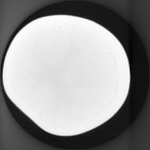
\includegraphics[width=\textwidth]{../images/potato/template_1.png}
\captionsetup{labelformat=empty}       
 \caption{}
    \end{subfigure}
    \begin{subfigure}[b]{0.24\linewidth}
        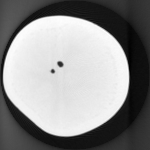
\includegraphics[width=\textwidth]{../images/potato/template_2.png}
\captionsetup{labelformat=empty}
        \caption{}
     \end{subfigure}
    \begin{subfigure}[b]{0.24\linewidth}
        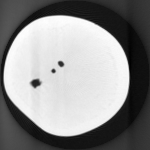
\includegraphics[width=\textwidth]{../images/potato/template_3.png}
\captionsetup{labelformat=empty}
        \caption{}
     \end{subfigure}
    \begin{subfigure}[b]{0.235\linewidth}
        \fcolorbox{yellow}{yellow}{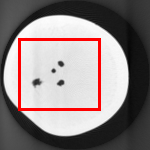
\includegraphics[width=\textwidth]{../images/potato/post_tci/testIm_paper.png}}
\captionsetup{labelformat=empty}
        \caption{}
\label{fig:potato_test}
     \end{subfigure}
      \caption{Potato dataset: One slice each from the previously scanned objects (the first three from left) and a slice from the test 
        volume (extreme right). Notice the appearance of the fourth
        hole in the test slice. }
\label{fig:object-prior_test_potato_A1}
\end{figure}
%-----------------------------potato 2D weights
\begin{figure}[!h]
    \begin{subfigure}[b]{0.24\linewidth}
        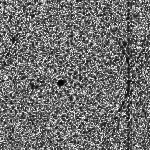
\includegraphics[width=\textwidth]{../images/potato/post_tci/comparison/weightsIm_fbp30.png}
        \caption{FBP}
    \end{subfigure}
    \begin{subfigure}[b]{0.24\linewidth}
        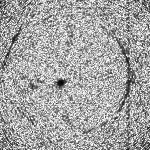
\includegraphics[width=\textwidth]{../images/potato/post_tci/comparison/weightsIm_cs_dct30.png}
        \caption{(l1-ls)-DCT}
     \end{subfigure}
    \begin{subfigure}[b]{0.24\linewidth}
        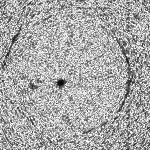
\includegraphics[width=\textwidth]{../images/potato/post_tci/comparison/weightsIm_cs_wavelet30.png}
        \caption{(l1-ls)-Haar}
     \end{subfigure}
    \begin{subfigure}[b]{0.24\linewidth}
        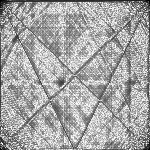
\includegraphics[width=\textwidth]{../images/potato/post_tci/comparison/weightsIm_art30.png}
        \caption{ART}
     \end{subfigure}
    \begin{subfigure}[b]{0.24\linewidth}
        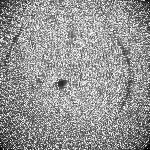
\includegraphics[width=\textwidth]{../images/potato/post_tci/comparison/weightsIm_sart30.png}
        \caption{SART}
     \end{subfigure}
    \begin{subfigure}[b]{0.24\linewidth}
        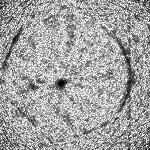
\includegraphics[width=\textwidth]{../images/potato/post_tci/comparison/weightsIm_sirt30.png}
        \caption{SIRT}
    \end{subfigure}
        \begin{subfigure}[b]{0.24\linewidth}
        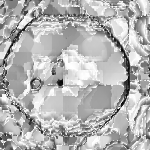
\includegraphics[width=\textwidth]{../images/potato/post_tci/comparison/weightsIm_tv30.png}
        \caption{TV}
     \end{subfigure}
    \begin{subfigure}[b]{0.24\linewidth}
        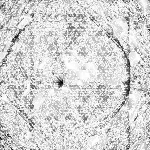
\includegraphics[width=\textwidth]{../images/potato/post_tci/comparison/weightsIm_all_methods30.png}
        \caption{combined}
     \end{subfigure}
      \caption{Weights-maps (corresponding to the difference between pilot reconstruction of the image in the last sub-figure of Fig.~\ref{fig:object-prior_test_potato_A1} and its projection onto the eigenspace $\boldsymbol{V_\text{low}}$) constructed using different reconstruction methods individually (a-f) and collectively (g) by fusing information from all reconstruction methods, as specified in Eq.~\ref{eq:weightsEq}. The weights-maps are different because the reconstruction artefacts of the new structures in test image will be different for every reconstruction method used, as seen in Fig.~\ref{fig:reconstructions_diff_methods}. }
\label{fig:weights_map_2Dpotato}
\end{figure}
%-----------------------------potato 2D weights
\begin{figure}[!h]
    \begin{subfigure}[b]{0.24\linewidth}
        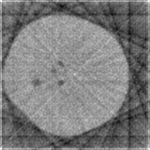
\includegraphics[width=\textwidth]{../images/potato/post_tci/comparison/fbp.png}
        \caption{FBP}
    \end{subfigure}
    \begin{subfigure}[b]{0.24\linewidth}
        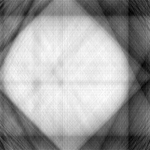
\includegraphics[width=\textwidth]{../images/potato/post_tci/comparison/cs_dct.png}
        \caption{(l1-ls)-DCT}
     \end{subfigure}
    \begin{subfigure}[b]{0.24\linewidth}
        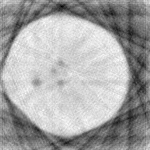
\includegraphics[width=\textwidth]{../images/potato/post_tci/comparison/cs_wavelet.png}
        \caption{(l1-ls)-Haar}
     \end{subfigure}
    \begin{subfigure}[b]{0.24\linewidth}
        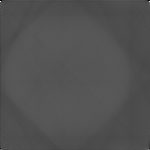
\includegraphics[width=\textwidth]{../images/potato/post_tci/comparison/art.png}
        \caption{ART}
     \end{subfigure}
    \begin{subfigure}[b]{0.24\linewidth}
        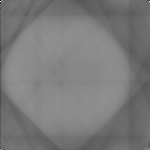
\includegraphics[width=\textwidth]{../images/potato/post_tci/comparison/sart.png}
        \caption{SART}
     \end{subfigure}
    \begin{subfigure}[b]{0.24\linewidth}
        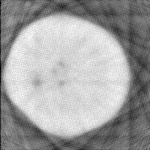
\includegraphics[width=\textwidth]{../images/potato/post_tci/comparison/sirt.png}
        \caption{SIRT}
    \end{subfigure}
        \begin{subfigure}[b]{0.24\linewidth}
        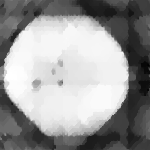
\includegraphics[width=\textwidth]{../images/potato/post_tci/comparison/tv.png}
        \caption{TV}
     \end{subfigure}
    \begin{subfigure}[b]{0.24\linewidth}
        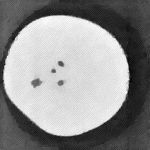
\includegraphics[width=\textwidth]{../images/potato/post_tci/comparison/weighted_pca_all_methods30.png}
        \caption{combined}
     \end{subfigure}
      \caption{(a)-(f):Different reconstructions of~\ref{fig:object-prior_test_potato_A1}(d). The magnitude and sharpness of the artefacts is different for each method. (g) Spatially-Varying-prior method that combines weights-map information from all other methods. The SSIM of these reconstructions is shown in Table.~\ref{table:potato_2D_ssim}.} 
\label{fig:reconstructions_diff_methods}
\end{figure}

The changes and new structures present in the test data will generate
different artifacts for different reconstruction techniques. These
artifacts would not be captured by reconstructions of the object-prior
since the underlying new changes and structures may be absent in all
of the previously scanned objects. We aim to let the weights be
independent of the type of artifact. Hence, we use a combination of
different reconstruction techniques to generate different types of
eigenspaces and combine information from all of them to compute
weights. To illustrate the benefit of this method, we first performed
2D reconstruction of a test slice from the potato dataset.
Fig.~\ref{fig:object-prior_test_potato_A1} shows the test and template
slices. Fig.~\ref{fig:weights_map_2Dpotato} shows the weights-maps
generated using Eq.~\ref{eq:weightsEq} by various reconstruction
methods. It can be seen that the weights are low in the region of the
new change in test data. Because all the iterative methods are
computationally expensive, we chose only FBP and (l1-ls)-DCT for
computing weights-maps for all 3D reconstructions.
%---------------------------------------
\begin{table}[!h]
  \centering
\caption{SSIM of the reconstructions shown in Fig.~\ref{fig:reconstructions_diff_methods}:(a)-(g). The SSIM of ground-truth (ideal reconstruction) is 1, and these are computed within the red RoI of the test image shown in Fig.~\ref{fig:potato_test}.}
\begin{tabular}{|l|c|c|c|c|c|c|c|c|c|}
\hline
 Fig.~\ref{fig:reconstructions_diff_methods}  & \textbf{(a)} & \textbf{(b)} & \textbf{(c)} & \textbf{(d)} & \textbf{(e)} & \textbf{(f)} &  \textbf{(g)} &  \textbf{(h)} \\\hline
\textbf{red RoI}  & 0.51 & 0.59  & 0.53 & 0.52 & 0.60 & 0.52 & 0.81 &\textcolor{red}{0.74} \\ \hline
\end{tabular}
\label{table:potato_2D_ssim}
\end{table}
%-------------------------------------------------

%----------------------------------------Results-----------------------
\section{Results: Reconstruction by spatially-varying prior}
\label{sec:results_spatially_varying_prior}

%The proposed method has been validated on 2D and 3D synthetic and real
%tomographic data of biological and medical specimens.
The results below show the advantage of spatially-varying prior over uniform prior while reconstructing details of the new changes within the object.

\subsubsection{\textbf{Okra}}
\label{Sec:okra_spatially_varying}
The test volume was reconstructed from a partial set of
45 projections, i.e., $10\%$ of the projection views from which ground
truth was reconstructed. One of the slices from the reconstructed volumes 
is shown in Fig.~\ref{fig:okra_3D_results}. The red and green 3D
RoI in the video and images show the regions where new changes are
present. The zoomed-in images around the major region of change (red
RoI) is shown in Fig.~\ref{fig:okra_zoomed_3D_results}. As in the
test, the reconstruction by spatially-varying method shows the absence
of the deformity and better removal of sub-sampling artefacts when
compared to FDK and l1-ls. This is also seen in the SSIM values in
Table~\ref{table:okra_ssim}.


\begin{figure}[!h]
\centering
\subcaptionbox{Test}{\fcolorbox{yellow}{yellow}{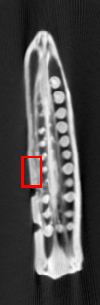
\includegraphics[width=0.23\columnwidth]{../images/okra/post_TCI/2D/48_views/input_roi.png}}}
\subcaptionbox{FBP, no prior}{\includegraphics[width=0.23\columnwidth]{../images/okra/post_TCI/2D/48_views/FBP_cropped.png}}
\subcaptionbox{TV, no prior}{\includegraphics[width=0.23\columnwidth]{../images/okra/post_TCI/2D/48_views/TV_cropped.png}}
%\subcaptionbox{\mbox{Uniform}\\prior}{\includegraphics[width=0.19\columnwidth]{../images/okra/pca_cropped.png}}\hfill
\subcaptionbox{Spatially-Varying\\ prior}{\includegraphics[width=0.23\columnwidth]{../images/okra/post_TCI/2D/48_views/weighted_prior_cropped.png}}
\caption{Reconstruction of 2D okra from 48 projection views
   (b) has streaky artefacts, (c) has blurred structures and (d) is sharper with significantly less streaky artefacts. The 3D reconstructed volumes can be viewed  in the supplementary material ~\cite{supp_paper}.}
\label{fig:okra_3D_results}
\end{figure}

%----------------------------------------------------

\begin{figure}[!h]
\centering
\subcaptionbox{Test}{\fcolorbox{yellow}{yellow}{\includegraphics[width=0.29\columnwidth]{../images/sprouts/post_TCI/2D/20_views/testIm_roi.png}}}
\subcaptionbox{FDK, no prior}{\includegraphics[width=0.3\columnwidth]{../images/sprouts/post_TCI/2D/20_views/fbp.png}}
\subcaptionbox{TV, no prior}{\includegraphics[width=0.3\columnwidth]{../images/sprouts/post_TCI/2D/20_views/tv_lambdaTV_0.100.png}}
%\subcaptionbox{\mbox{Uniform}\\prior}{\includegraphics[width=0.19\columnwidth]{../images/okra/pca_cropped.png}}\hfill
\subcaptionbox{Spatially-Varying\\ prior}{\includegraphics[width=0.3\columnwidth]{../images/sprouts/post_TCI/2D/20_views/weighted_prior_kk_30_lambda_prior_2.100000.png}}
\caption{Reconstruction of 2D sprouts from 20 projection views
   (b) has streaky artefacts, (c) has blurred structures and (d) is sharper with significantly less streaky artefacts. The 3D reconstructed volumes can be viewed  in the supplementary material ~\cite{supp_paper}.}
\label{fig:sprouts3D_results}
\end{figure}


%---------------------------------------
\begin{table}[!h]
  \centering
  \caption{SSIM of reconstructed okra from various
    methods. For 3D, the RoI spans 7 consecutive slices where the test is
    different from all of the previously scanned objects. The SSIM of ground-truth (ideal reconstruction) is 1.}
\begin{tabular}{|l|c|c|c|c|c|}
\hline &
\textbf{Backprojection} & \textbf{TV} &
\textbf{\begin{tabular}[c]{@{}c@{}}Spatially Varying\\prior +
    TV\end{tabular}} \\ \hline \textbf{2D} & 0.46
& 0.50 & \textcolor{red}{0.74} \\ \hline \textbf{3D} & 0.69 & 0.74 & \textcolor{red}{0.78}
\\ \hline
\end{tabular}
\label{table:okra_ssim}
\end{table}



\subsubsection{\textbf{Sprouts}}
\label{Sec:sprouts_spatially_varying}
 %-----------------------------sprouts 3D results

%--------------------------------------------------------------
\begin{table}[!h]
  \centering
  \caption{SSIM of reconstructed sprouts from various
    methods. For 3D, the RoI spans 7 consecutive slices where the test is
    different from all of the previously scanned objects. The SSIM of ground-truth (ideal reconstruction) is 1.}
\begin{tabular}{|l|c|c|c|c|c|}
\hline &
\textbf{Backprojection} & \textbf{TV} &
\textbf{\begin{tabular}[c]{@{}c@{}}Spatially Varying\\prior +
    TV\end{tabular}} \\ \hline \textbf{2D} & 0.67
& 0.82 & \textcolor{red}{0.86} \\ \hline \textbf{3D} & 0.67 & 0.73 & \textcolor{red}{0.82}
\\ \hline
\end{tabular}
\label{table:sprouts_ssim}
\end{table}


The test volume was reconstructed from partial set of 45
projections, i.e., $2.5\%$ of the projection views from which ground
truth was reconstructed. The selected 3D ground truth of
template volumes, test volume, as well as the 3D reconstructions are
shown in the supplementary material~\cite{supp_paper}. One of the slices of the reconstructed
volumes and its zoomed-in RoI are shown in
Figs.~\ref{fig:sprouts_3D_results} and
~\ref{fig:sprouts_zoomed_3D_results} respectively. For the sake of
exposition, the red region of interest (RoI) has been culled out from
7 consecutive slices in the 3D volume to indicate new structures;
other changes can be viewed in the video. Tables~\ref{table:okra_ssim}
and \ref{table:sprouts_ssim} show the improvement in SSIM of the reconstructed new regions as compared
to other methods.

%--------------------------------------------------------------------------


\section{Discussion}
\label{sec:discussion}
In this section, we discuss the following:  a) an alternate imaging and reconstruction protocol for longitudinal studies, b) results on homogeneous dataset, and (c) tuning of the parameters used.
%The presented uniform prior-based algorithm is suited to applications
%where we wish to detect the location of new changes in an object over
%time, and the presented spatially-varying prior-based algorithm is
%suited to applications where we wish to observe the intricate details
%of those new changes. %This distinction in the techniques used has not
%been studied earlier in
%literature~\cite{geyer2015,PICCS,Ali2018,Tan2017} to the best of our
%knowledge. Even though methods such as~\cite{Hakka2019} offer the flexibility of using multiple templates, the very important issue of these templates overwhelming the current reconstruction has been largely ignored. We have presented a principled method of tackling this particular issue via our weights map. We not only estimate the location of new changes, but also compute their intensities. This information is then used to modulate the strength of the prior during the reconstruction of the test. Our results consist of 3D reconstructions from real cone-beam projections of two datasets, and both 3D and 2D reconstructions from cone-beam and parallel beam projections respectively. In each case, we have compared our results with those from standard back-projection algorithms~\cite{Pan2009} (FDK in case of 3D and FBP incase of 2D), and Compressed Sensing~\cite{Donoho,introCS} based reconstructions. An in-depth analysis of each of the results is presented in Sections~\ref{sec:results_uniform_prior} and~\ref{sec:results_spatially_varying_prior}. We now discuss computation times, the method that suits best when the data is homogeneous, and the effect of hyper-parameters on our reconstructions.

%-----------------------------------------


\subsection{Reconstruction of homogeneous data}
\label{Sec:potato}
%--------potato reconstruction--------------------------------------------------
\begin{figure}[!h]
\centering
\subcaptionbox{Test}{\fcolorbox{blue}{blue}{\includegraphics[width=0.22\columnwidth]{../images/potato/post_tci/testIm_paper.png}}}
\subcaptionbox{FDK, no prior}{\includegraphics[width=0.23\columnwidth]{../images/potato/post_tci/6_views/fbp.png}}
\subcaptionbox{TV, no prior}{\includegraphics[width=0.23\columnwidth]{../images/potato/post_tci/6_views/tv_lambdaTV_0.05.png}}
\subcaptionbox{Spatially-Varying\\ prior}{\includegraphics[width=0.23\columnwidth]{../images/potato/post_tci/6_views/weighted_prior_kk_30_lambda_prior_1.100000.png}}
\caption{Reconstruction of the 2D-potato from 6 projection views--(b) has strong streak artefacts with unclear structure of the potato, (c) largely blurred, and (c) is sharper with significantly reduced streak artefacts. The 3D reconstructed volumes can be viewed in the supplementary material~\cite{supp_paper}.}
\label{fig:potato_3D_results_A}
\end{figure}
%-------------------------------------------------------------------------
\begin{table}[!h]
  \centering
  \caption{SSIM of reconstructed potato from various
    methods. For 3D, the RoI spans 7 consecutive slices where the test is
    different from all of the previously scanned objects. The SSIM of ground-truth (ideal reconstruction) is 1.}
\begin{tabular}{|l|c|c|c|c|c|}
\hline &
\textbf{Backprojection} & \textbf{TV} &
\textbf{\begin{tabular}[c]{@{}c@{}}Spatially Varying\\prior +
    TV\end{tabular}} \\ \hline \textbf{2D} & 0.52
& 0.92 & \textcolor{red}{0.97} \\ \hline \textbf{3D} & 0.58 & 0.75 & \textcolor{red}{0.84}
\\ \hline
\end{tabular}
\label{table:potato_ssim}
\end{table}


While the design of the weights map in the proposed algorithm aims to
combine the best of information from both the current measurements and
the prior, we found FDK to be preferable when the test object has a
simple, homogeneous structure without intricate details. One such
dataset is the Potato dataset (described in
Sec.~\ref{sec:datasets}). The test volume was reconstructed using
measurements from 45 projection views, i.e., $5\%$ of the projection
views from which ground truth was reconstructed. The selected 3D
ground truth of template volumes, test volume, as well as the 3D
reconstructions are shown in the supplementary
material~\cite{supp_paper}. Fig.~\ref{fig:potato_3D_results_A} shows a
slice from the reconstructed 3D volume. We observe that our method
reconstructs new structures while simultaneously reducing streak
artefacts. Table~\ref{table:potato_ssim} shows the Structure Similarity
Index (SSIM) of the reconstructed new regions using various
methods. We observe that FDK performs very well for smaller RoI;
as the RoIs get bigger, the FDK reconstructions have poor SSIM due to
strong subsampling artefacts. In contrast, the results from l1-ls and
our method progressively improve when compared to FDK as the RoIs get
bigger. In practice, the RoI is not known in advance and hence, one
may choose FDK for the case of simple, homogeneous dataset with
smaller RoI, and prefer spatially-varying prior-based reconstruction
when the dataset is complex and RoIs are larger.

%The new regions detected by different reconstruction methods are shown in Fig.~\ref{fig:weights_map_2Dpotato}. The lower intensities denote new regions which were assigned lower weights. This ensures that the new regions are reconstructed using projection measurements alone, avoiding erroneous influence of the prior.

\subsection{Tuning of parameters}
\label{subsec:k}
 $\lambda_1$ was tuned to maximize
SSIM of the whole reconstructed test volume for l1-ls reconstruction
of each dataset. This value was retained for uniform and
spatially-varying prior-based reconstruction as well. The value of
$\lambda_2$ largely depends on the amount of artefacts we aim to
remove by using prior at the cost of their dominance in the new
regions. This value was chosen to lie between $0-1$ for our
datasets. Finally, the hyper-parameter $k$ defines the sensitivity of
the weights map to the difference between the test image and the prior
(projection of test onto the space of object-prior). When $k=0$, our
method converges to the uniform prior method. As $k$ increases, the
weights map starts capturing the new changes in the test, at the cost
of detecting a few false positives i.e., false new changes. In other
words, as the weights map becomes more sensitive to the difference
between the test and object-prior, it becomes more noisy. In order to
visualize the effect of the hyper-parameter $k$, we performed 2D
reconstructions of okra dataset for different values of
$k$. Fig.~\ref{fig:few_view_okra_2D_weights} shows the weights map
obtained for each of the $k$ values. We estimate an approximate choice
for the optimal value of $k$ by treating one of the object-prior as
test and reconstructing it. We also note that although the weights map
is heavily influenced by $k$, the final reconstructions are stable for
large variations in $k$, as seen in
Fig.~\ref{fig:reconstructions_as_k_varies}. Alternatively, in cases
where one wishes to completely avoid the use of this hyper-parameter,
one can construct a binary weights-map using a learning based method
described in the supplementary material~\cite{supp_paper}.

%--------------effect of the value of $k$ on Okra dataset


\begin{figure}[h]
    \begin{subfigure}[b]{0.24\linewidth}
        \includegraphics[width=\textwidth]{../images/okra/post_TCI/2D/48_views/tuning_k/weightsIm_kk_5_lambda_prior_0.700000.png}
        \caption{k=5}
     \end{subfigure}     
  \begin{subfigure}[b]{0.24\linewidth}
        \includegraphics[width=\textwidth]{../images/okra/post_TCI/2D/48_views/tuning_k/weightsIm_kk_10_lambda_prior_0.700000.png}
        \caption{k=10}
     \end{subfigure} 
  \begin{subfigure}[b]{0.24\linewidth}
        \includegraphics[width=\textwidth]{../images/okra/post_TCI/2D/48_views/tuning_k/weightsIm_kk_20_lambda_prior_0.700000.png}
        \caption{k=20}
     \end{subfigure}
  \begin{subfigure}[b]{0.24\linewidth}
        \includegraphics[width=\textwidth]{../images/okra/post_TCI/2D/48_views/tuning_k/weightsIm_kk_30_lambda_prior_0.700000.png}
        \caption{k=30}
     \end{subfigure}
  \begin{subfigure}[b]{0.24\linewidth}
        \includegraphics[width=\textwidth]{../images/okra/post_TCI/2D/48_views/tuning_k/weightsIm_kk_40_lambda_prior_0.700000.png}
        \caption{k=40}
     \end{subfigure}
  \begin{subfigure}[b]{0.24\linewidth}
        \includegraphics[width=\textwidth]{../images/okra/post_TCI/2D/48_views/tuning_k/weightsIm_kk_50_lambda_prior_0.700000.png}
        \caption{k=50}
     \end{subfigure}
   \begin{subfigure}[b]{0.24\linewidth}
        \includegraphics[width=\textwidth]{../images/okra/post_TCI/2D/48_views/tuning_k/weightsIm_kk_60_lambda_prior_0.700000.png}
        \caption{k=60}
     \end{subfigure}
   \begin{subfigure}[b]{0.24\linewidth}
        \includegraphics[width=\textwidth]{../images/okra/post_TCI/2D/48_views/tuning_k/weightsIm_kk_70_lambda_prior_0.700000.png}
        \caption{k=70}
     \end{subfigure}
  \begin{subfigure}[b]{0.24\linewidth}
        \includegraphics[width=\textwidth]{../images/okra/post_TCI/2D/48_views/tuning_k/weightsIm_kk_80_lambda_prior_0.700000.png}
        \caption{k=80}
     \end{subfigure}
   \begin{subfigure}[b]{0.24\linewidth}
        \includegraphics[width=\textwidth]{../images/okra/post_TCI/2D/48_views/tuning_k/weightsIm_kk_90_lambda_prior_0.700000.png}
        \caption{k=90}
     \end{subfigure}
   \begin{subfigure}[b]{0.24\linewidth}
        \includegraphics[width=\textwidth]{../images/okra/post_TCI/2D/48_views/tuning_k/weightsIm_kk_100_lambda_prior_0.700000.png}
        \caption{k=100}
     \end{subfigure}
   \begin{subfigure}[b]{0.24\linewidth}
        \includegraphics[width=\textwidth]{../images/okra/post_TCI/2D/48_views/tuning_k/weightsIm_kk_130_lambda_prior_0.700000.png}
        \caption{k=130}
     \end{subfigure}
    \caption{Different weights-maps for okra reconstruction. Low intensity denotes regions of new changes in test.}
\label{fig:few_view_okra_2D_weights}
\end{figure}
\begin{figure}[h]
    \begin{subfigure}[b]{0.24\linewidth}
        \includegraphics[width=\textwidth]{../images/okra/post_TCI/2D/48_views/tuning_k/weighted_prior_kk_5_lambda_prior_0.700000.png}
        \caption{k=5,\\ SSIM = 0.79}
     \end{subfigure}     
  \begin{subfigure}[b]{0.24\linewidth}
        \includegraphics[width=\textwidth]{../images/okra/post_TCI/2D/48_views/tuning_k/weighted_prior_kk_10_lambda_prior_0.700000.png}
        \caption{k=10,\\ SSIM = 0.78}
     \end{subfigure} 
  \begin{subfigure}[b]{0.24\linewidth}
        \includegraphics[width=\textwidth]{../images/okra/post_TCI/2D/48_views/tuning_k/weighted_prior_kk_20_lambda_prior_0.700000.png}
        \caption{k=20,\\ SSIM = 0.76}
     \end{subfigure}
  \begin{subfigure}[b]{0.24\linewidth}
        \includegraphics[width=\textwidth]{../images/okra/post_TCI/2D/48_views/tuning_k/weighted_prior_kk_30_lambda_prior_0.700000.png}
        \caption{k=30,\\ SSIM = 0.74}
     \end{subfigure}
  \begin{subfigure}[b]{0.24\linewidth}
        \includegraphics[width=\textwidth]{../images/okra/post_TCI/2D/48_views/tuning_k/weighted_prior_kk_40_lambda_prior_0.700000.png}
        \caption{k=40,\\ SSIM = 0.72}
     \end{subfigure}
  \begin{subfigure}[b]{0.24\linewidth}
        \includegraphics[width=\textwidth]{../images/okra/post_TCI/2D/48_views/tuning_k/weighted_prior_kk_50_lambda_prior_0.700000.png}
        \caption{k=50,\\ SSIM = 0.63}
     \end{subfigure}
   \begin{subfigure}[b]{0.24\linewidth}
        \includegraphics[width=\textwidth]{../images/okra/post_TCI/2D/48_views/tuning_k/weighted_prior_kk_60_lambda_prior_0.700000.png}
        \caption{k=60,\\ SSIM = 0.61}
     \end{subfigure}
   \begin{subfigure}[b]{0.24\linewidth}
        \includegraphics[width=\textwidth]{../images/okra/post_TCI/2D/48_views/tuning_k/weighted_prior_kk_70_lambda_prior_0.700000.png}
        \caption{k=70,\\ SSIM = 0.59}
     \end{subfigure}
  \begin{subfigure}[b]{0.24\linewidth}
        \includegraphics[width=\textwidth]{../images/okra/post_TCI/2D/48_views/tuning_k/weighted_prior_kk_80_lambda_prior_0.700000.png}
        \caption{k=80,\\ SSIM = 0.58}
     \end{subfigure}
   \begin{subfigure}[b]{0.24\linewidth}
        \includegraphics[width=\textwidth]{../images/okra/post_TCI/2D/48_views/tuning_k/weighted_prior_kk_90_lambda_prior_0.700000.png}
        \caption{k=90,\\ SSIM = 0.56}
     \end{subfigure}
   \begin{subfigure}[b]{0.24\linewidth}
        \includegraphics[width=\textwidth]{../images/okra/post_TCI/2D/48_views/tuning_k/weighted_prior_kk_100_lambda_prior_0.700000.png}
        \caption{k=100,\\ SSIM = 0.55}
     \end{subfigure}
   \begin{subfigure}[b]{0.24\linewidth}
        \includegraphics[width=\textwidth]{../images/okra/post_TCI/2D/48_views/tuning_k/weighted_prior_kk_130_lambda_prior_0.700000.png}
        \caption{k=130,\\ SSIM = 0.53}
     \end{subfigure}
    \caption{2D reconstructions for varying values of $k$. The SSIM values for all images are computed within the red RoI (shown in Fig.~\ref{fig:okra_3D_results}(a)), the region where the test is different from all of the previously scanned objects.}
\label{fig:reconstructions_as_k_varies}
\end{figure}


%--------------------------Conclusion-----------------------
\section{Conclusions}
\label{sec:conclusions}
This work deals with the effective use of priors for tomographic
reconstruction in longitudinal studies. We show that we can either use
the uniform prior method or the spatially-varying prior method to our
advantage, depending on our goal. We establish the context under which
these methods can be used, as outlined in
Fig.~\ref{fig:prior_overview}. When we wish to approximately know the
location of new changes, we apply a uniform prior because it is
sufficient for the task at hand. We also choose a smaller number
of views in order to reduce radiation. In addition, we show that when
our goal shifts to observing the details of the new changes
accurately, we acquire projections from a moderate number of views in
order to capture more information. We further combine this with the
somewhat slower but more accurate technique of reconstruction-- the
spatially-varying prior-based method. This method ensures that the
reconstruction of localized new information in the data is not
affected by the priors. %Based on the potato and the okra experiments,
%we see that our method is able to \emph{discover both} the presence of
%a new structure, as well as the absence of a structure.
We have thus
improved the state of the art by detecting these regions of change and
assigning low prior weights wherever necessary. The probability of
presence of a `new region' is enhanced considerably by a novel
combination of different reconstruction techniques.  We have validated
our technique on medical 2D and real, biological 3D datasets for
longitudinal studies. The method is also largely robust to the number
of previously scanned objects used. We urge the reader to see the
videos of reconstructed volumes in the supplementary
material~\cite{supp_paper}.
%Our method has been shown to make the best use of prior
%only when needed, thus detecting new changes of the test
%data. 

\section{Acknowledgement}
We are grateful to Dr. Andrew Kingston for facilitating data
collection at the Australian National University. AR gratefully
acknowledges IITB Seed-grant 14IRCCSG012, as well as NVIDIA
Corporation for the generous donation of a Titan-X GPU card, which was
essential for computing 3D reconstructions for the research reported
here. We also thank Dr. Akshay Baheti for providing us with medical
data from Tata Memorial Hospital, Mumbai.
{%\footnotesize
\bibliography{tci_ref}}
\end{document}

